\documentclass[11pt, letterpaper, titlepage]{article}
\usepackage[utf8]{inputenc}
\usepackage[export]{adjustbox}
\usepackage{geometry}
 \geometry{
 a4paper,
 total={168mm,257mm},
 left=20mm,
 top=15mm,
 includefoot,includehead
 }

\usepackage{siunitx}
\usepackage[backend=biber, style=authoryear, giveninits=true, maxbibnames=25, uniquename=init, maxcitenames=2, hyperref=true, dashed=false]{biblatex}			% Benutze Biber/BibLaTeX zum Zitieren
\addbibresource{main.bib}					% Pfad zur BibTeX Datei aus Citavi
\renewcommand{\cite}{\parencite}
\usepackage{caption}
\usepackage{subcaption}
\usepackage{graphicx}
\usepackage{svg}
\usepackage{placeins}
\usepackage[hidelinks]{hyperref}
\usepackage{amsmath}
\usepackage[headsepline]{scrlayer-scrpage}
\usepackage{acronym}

\clearpairofpagestyles %Seitenzahl nicht in der Kopfzeile

\title{MeetEU Project - Team Heidelberg - Team 1 -- \\ Identification and Enhancement of novel Sars-CoV-2 NSP13 Helicase Inhibitors}
\author{Linda Blaier, Paul Brunner, Selina Ernst, Valerie Segatz, and Chlo\'{e} Weiler}
\date{February 2024}

\begin{document}

\maketitle

\ihead{\headmark}
\automark{section}  %Kopfzeile gleich dem Sektiontitel
\cfoot{\pagemark}   %\ofood Seitenzahl rechts



\section{Abstract}
Although the development of vaccines against Sars-CoV-2 was successful during the recent pandemic, the amount of FDA approved drugs for the therapy of Covid-19 is still limited to Paxlovid and Veklury, Olumiant and Actemra \cite{FDACOVID}. One possibility to accelerate the development of new therapies for Covid19 is to screen already approved drugs for effects against the viral reproduction. In this years MeetEU project, we investigated the NSP13 helicase of Sars-CoV-2 and tried to find compounds that could be repurposed for this therapy, as well as novel compounds that could lead to an effective treatment of Covid19. Using our \textit{in-silico} pipeline (see graphical abstract) enables us to evaluate possible drug candidates, suggest novel structures based on already approved drugs and investigate their toxicity, while being cheaper and less labor intensive than projects limited to wet-lab work.\\
\FloatBarrier

\begin{figure}[h]
  \centering
  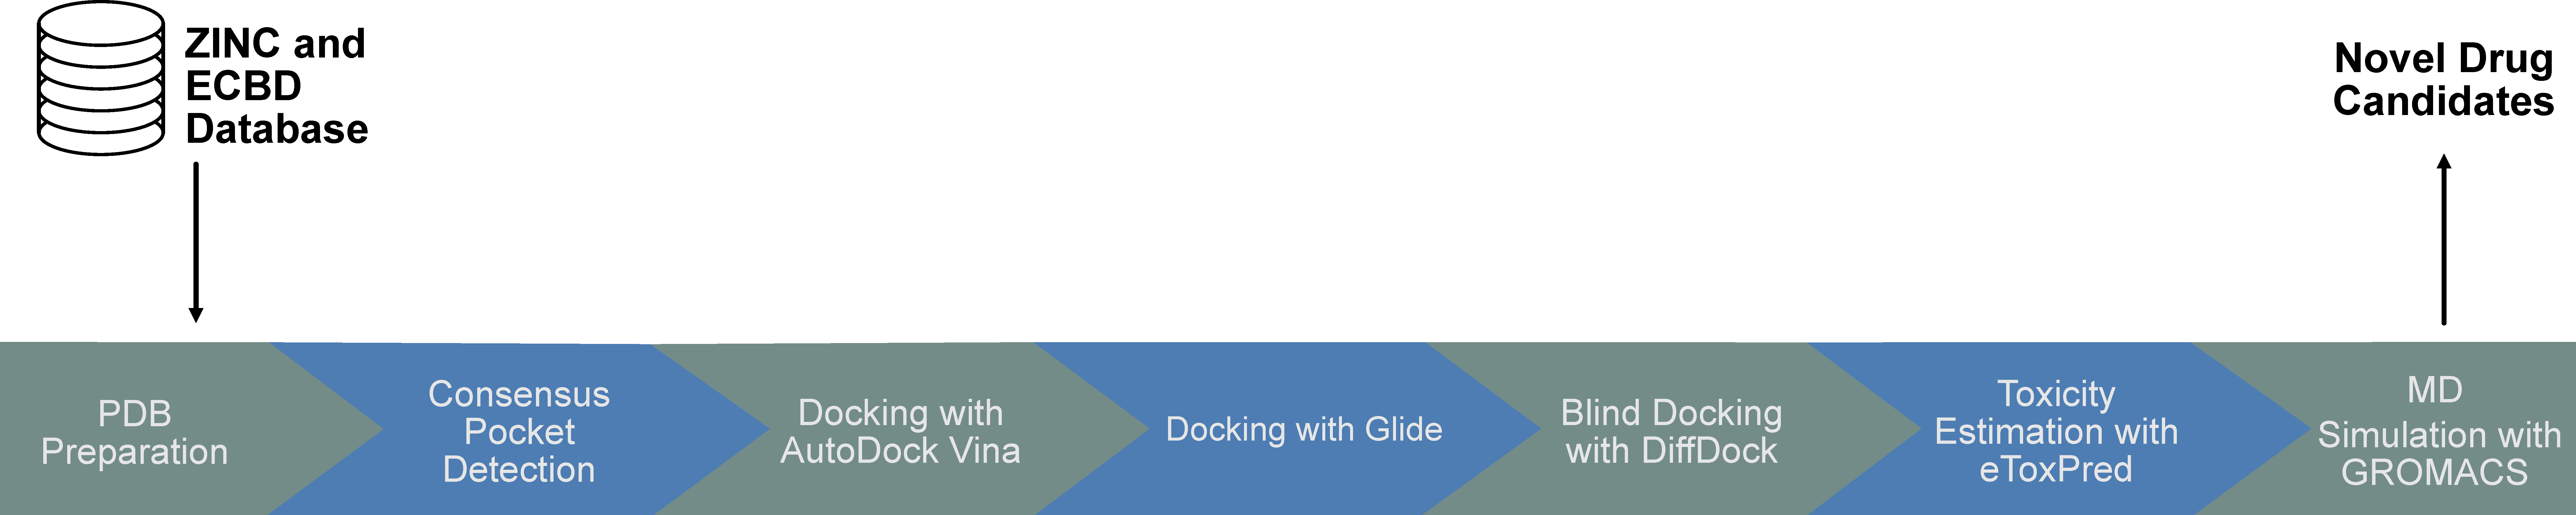
\includegraphics[width=\textwidth]{Workflow_MeetEU.pdf}
  \caption*{Proposed workflow for the discovery of NSP13 helicase inhibitors.}
  \label{workflow}
\end{figure}

\setcounter{figure}{0}
\renewcommand{\thefigure}{\arabic{figure}}
\newpage

%    Abkürzungsverzeichnis
{\setlength{\parskip}{0.2cm}
\section*{Abbreviations}
    \begin{acronym}[LC-MS/MS23]
        % A B C D E F G H I J K L M N O P Q R S T U V W X Y Z        
        % Abkürzungen
    \acro{ADP}{adenosine diphosphate}
    \acro{ATP}{adenosine triphosphate}
    \acro{COVID-19}{coronavirus disease 2019}
    \acro{FDA}{food and drug administration}
    \acro{MD}{molecular dynamics}
    \acro{MM-PBSA}{molecular mechanics energies combined with the Poisson-Boltzmann and surface area continuum solvation}
    \acro{NSP13}{non-structural protein 13}
    \acro{RCSB PDB}{Research Collaboratory for Structural Bioinformatics Protein Data Bank}
    \acro{RMSD}{root mean square deviation}
    \acro{RMSF}{root mean square fluctuation}
    \acro{RTC}{replication transcription complex}
    \acro{SARS-CoV-2}{severe acute respiratory syndrome coronavirus type 2}
    \acro{SAscore}{synthetic accessibility score}
    \acro{ssRNA}{single-stranded RNA}
    \acro{ZBD}{zinc-binding domain}
       
        % Formelzeichen
        
        
        % als benutzt markierte Acronyme    
        
        
    \end{acronym}
}
\newpage

\section{Introduction}
In the wake of the successful development of vaccines against \ac{SARS-CoV-2} during the recent pandemic, the amount of FDA-approved drugs for the therapy of \ac{COVID-19} remain limited to Paxlovid, Veklury, Olumiant, and Actemra \cite{FDACOVID}. Expanding the repertoire of drugs available for treating \ac{COVID-19} is particularly crucial for high-risk individuals, as vaccines may not fully prevent infections. The goal of this year's Meet-EU project is to develop a pipeline for identifying potential inhibtiors targeting the SARS-CoV-2 helicase also known as \ac{NSP13}. 
This protein is considered a promising drug target for two reasons. Firstly, \ac{NSP13} is part of the \ac{RTC} which is essential for viral RNA synthesis \cite{Malone_2022}. Secondly, its high conservation across coronaviruses means that there is a reduced likelihood of the virus developing resistances to drugs targeting \ac{NSP13} through mutations of the viral genome \cite{Spratt_2021}. Consequently, effective \ac{NSP13} inhibition would significantly impede viral replication and therefore its spread within the host. 
\ac{NSP13} consists of five domains, namely the \ac{ZBD} with the accessory 2B domain, the $\alpha$-helical stalk domain, as well as the RecA-like 1A and 2A domains \cite{Marecki}. The gap between the RecA-like domains and the 2B domain encompass the site for ATP and RNA binding \cite{NSP13_basics}. In the \ac{RTC} the NSP13 helicase is present as a homodimer. Nevertheless, only one of the copies complexes with a single-stranded RNA \ac{ssRNA}. Therefore, it was proposed in previous publications that the catalytically active form of the \ac{NSP13} helicase is the monomer \cite{Berta_2021}. \\

\noindent Computer-aided, structure-based drug discovery is employed for identification of known drugs for their potential as inhibitors of the \ac{NSP13} helicase which can then be further investigated in experimental laboratory settings. This process involves several steps: (i) Identification of potential drug binding sites, (ii) high-throughput screening of ligands to assess their binding efficacy within the  designated pocket, followed by (iii) the evaluation of the binding pathways, kinetics, and thermodynamics \cite{Sledz_2018}. Focussing this screening on well-documented or already FDA-approved compounds is very attractive, as drug repurposing has the potential to shorten the development period and therefore also the development costs \cite{Pushpakom_2019}.

%To explore new therapy options it makes sense to perform a  \textit{in-silico} screening of different compounds to identify groups that interact well with the \ac{NSP13} helicase. This screening process involves several steps: Identify possible binding sites, screen ligands for how well they bind in this pocket and validate the findings to generate a suggestion, as to which compounds would be worth it to investigate in a wet-lab setting \cite{Sledz_2018}. Focussing this screening on well documented or already FDA approved compounds significantly simplifies a potential registration of a potential new drug entering the market. 

\subsection{Identification of Consensus Binding Pocket}
In drug discovery, the initial step is to investigate the protein structure in order to analyse potential binding sites. These are cavities on the surface or interior of the protein with suitable properties to bind a ligand. The functionality of a binding pocket is determined by its shape and location, but also by the amino acid residues which define its pyhsicochemical characteristics \cite{Stank_2016}. 
Different experimental and theoretical procedures exist to analyse the druggability of such binding pockets. In this work, we combined three different \textit{in silico} tools, each following a different algorithm. \textit{Fpocket} \cite{package_Fpocket} utilises a geometry-based algorithm based on Voronoi tesselation and sequential clustering to determine potential binding sites. We also used PRankweb which is the web interface based on the P2Rank standalone method which is based on a machine-learning algorithm \cite{package_P2Rank, package_PrankWeb, package_PrankWeb3}. 
P2Rank assigns structural, physicochemical, and evolutionary features to points on the solvent-accessible surface of a protein. From this information, the machine-learning model is built and used to predict and rank potential ligand binding sites. Lastly, FTMAP \cite{package_FTMAP} was used to validate the binding pocket found with the previously mentioned approaches. FTMAP uses docking results of sixteen small molecules differing in polarity, shape, and size to identify binding hot spots with a fast Fourier transform correlation. The most favourable docked confirmations are determined through energy minimisation and clustering processes.
Finally, the results of all three tools were combined to identify a consensus binding pocket of the NSP13 helicase. The resulting coordinates of the consensus binding pocket were then used for molecular docking simulations. 

\subsection{Molecular Docking}
Molecular Docking programs are used to evaluate binding affinities between a potential drug candidate and the target protein. A key aspect of this task is the prediction of the ligand position, orientation, and conformation. Search-based methods approach this task by continuously modifying the ligand pose, while estimating its quality or likelihood (score) and stochastically trying to infer the global optimum of the scoring function. Among the most widely used tools are \textit{AutoDock Vina} \cite{Trott.2010} and \textit{Glide} \cite{Halgren.2004}, which mainly differ in their scoring functions. However, such search-based methods are computationally expensive. Therefore, in order to be able to screen large datasets, search-based methods are generally restricted to a previously defined binding pocket \cite{Corso.2022}. Consequently, potential other binding sites of a ligand are not assessed. Machine learning-based blind docking approaches try to address that problem by stochastically predicting binding pocket and ligand pose based on learned characteristics and aligning them. The most promising results are achieved by using \textit{Diffdock} \cite{Corso.2022}, a generative model which applies a reverse diffusion process to the docking paradigm. In this manner, \textit{Diffdock} iteratively transforms an uninformed noisy distribution over ligand poses defined by the degrees of freedom involved in docking (position, turns around its centre of mass, and twists of torsion angles) into a learned model distribution \cite{Corso.2022}. \citeauthor{Corso.2022} thereby describe this process as a progressive refinement of random ligand poses via updates of their translations, rotations and torsion angles.

%\subsection{Lead Drug Enhancement}
%In order to enhance the binding affinity of our drug candidates and thus their performance, we used AutoGrow4 (Version 4.0.3) \cite{package_Autogrow4} to generate novel compounds. Starting with the best binding compounds of our initial docking simulation with AutoDock Vina as generation zero, multiple new structures are generated by combining sub-structures of the first generation or by passing them through a set of possible chemical reactions after converting them into their respective SMILES codes. All of the generated compounds are ranked by their binding affinity. After passing several filters, the best-performing compounds are used as the seed for the next generation. Using this algorithm, compounds are found, which show higher binding affinities than the first generation. As AutoGrow4 labels all new structures by the path by which they were obtained, we can also evaluate the synthesizability.  

\subsection{Estimation of Toxicity and Synthetic Accessibility}
After identifying the lead compounds that exhibit optimal binding affinity within the consensus pocket, an evaluation of the general toxicity and synthetic accessibility of these compounds was performed using the latest version of \textit{eToxPred} \cite{pu2019toxpred}. This additional step helps estimate the suitability of the compounds as real-life pharmaceuticals against COVID-19. The Tox-score allows for a general assessment of the predicted risk vs. benefit ratio of the potential NSP13 inhibitors. Moreover, \textit{eToxPred} allows for an insight into the ease of synthesis, indicated by the synthetic accessibility score \ac{SAscore}. This score reflects the ease and efficiency of producing the molecules in large quantities and consequently their feasibility as potential drugs. 

\subsection{Molecular Dynamics Simulation}
As the last step of our pipeline, an \ac{MD} simulation is conducted using the best-scoring compounds as a ligand in the binding pocket of the \ac{NSP13} protein. Simulating the movement of molecules in a system based on the attractive and repulsive forces between atoms helps with understanding the molecular interplay between the found ligands and the binding pocket. Whether the ligand stays inside  the binding pocket throughout the whole simulation gives an estimate of how strongly it binds to the protein \cite{MD_Basics}. As this is the final step of our pipeline, the result of this simulation estimates how the ligand would perform if administered \textit{in-vitro}. Additionally, the frames generated by the software can be used to calculate different metrices regarding the binding strength, like the \ac{RMSF}, \ac{RMSD} and the binding affinities estimated by \ac{MM-PBSA}. The \ac{RMSD} measures the average displacement of the atoms throughout the simulation compared to the first frame of the simulation and estimates how much the protein moves and changes conformations over time. The \ac{RMSF} on the other hand calculates the movement of a certain atom or group of atoms over time compared to the average position of the atoms and groups \cite{RMSD_RMSF}. \ac{MM-PBSA} is able to estimate the binding affinity of the simulated protein-ligand pair \cite{MM_PBSA}.


\section{Material and Methods}
\subsection{Datasets from ZINC20 and ECBD}
A total of 1616 \ac{FDA}-approved drugs were downloaded in \textit{.sdf} format from the ZINC database \cite{Irwin.2020}. Additionally, 5016 files were retrieved, downloading the pilot library from the ECBD database.

\subsection{Receptor and Ligand Preparation}
In this project we analysed crystal structures of the \ac{SARS-CoV-2} \ac{NSP13} helicase which were obtained by \cite{NSP13_basics} in a crystallographic fragment screening. Thus, the three protein structures (PDB codes: 6ZSL, 5RME, 5RM2) were downloaded from the protein data bank \ac{RCSB PDB}. All three structures were used to determine a consensus binding pocket. As 6ZSL is the crystal structure with the highest resolution of 1.94 {\AA} and the other two structures show the \ac{NSP13} helicase complexed with a different fragment, we selected 6ZSL for further analysis in our drug discovery pipeline. Although the helicase is a homodimer, it was found that only the monomer is the catalytically active form \cite{Berta_2021}. Therefore, we concentrated our drug discovery only on the monomer of the helicase, namely on chain A. \\
Protein Data Bank (PDB) files often contain problems that first need to be resolved so they can be used for further simulations. Therefore, we prepared the PDB protein structure using the \textit{PDBFixer} (Version 1.9) application, which among other things adds missing hydrogen and heavy atoms, builds missing loops and replaces non-canonical with canonical amino acids \cite{Eastman_2017}. Here, we added hydrogen atoms appropriate for the physiological pH of 7.4. The B chain of 6ZSL, identical to the A chain, contained in the crystallographic structure was removed as well as all phosphates and the ligands contained in the protein structures of 5RME and 5RM2. Additionally, for molecular docking using \textit{AutoDock Vina} %add citation here --> (Version 1.1.2, henceforth abbreviated as Vina, \textcite{Trott.2010}) but how should we handle the henceforth then?
and for the \ac{MD} simulation the zinc ions were removed. For consensus binding site detection 6ZSL was used as a reference structure to align 5RME and 5RM2 in \textit{PyMol} (Version 2.5.7, \textcite{PyMol_endnote}).This allowed better visualization and superimposition of the results.\\ 
Ligands were prepared using \textit{OpenBabel} (Version 3.1.1, \textcite{OpenBabel}) in order to convert implicit hydrogens into explicit hydrogens, to generate the necessary 3D structures of the ligands, and to split multi-molecule files into single ones. \textit{ADFR suite} (Version 1.0, \textcite{AutoDockFR}) was further used in order to convert all files into the \textit{.pdbqt} format, which is required by \textit{Autodock Vina} \cite{Trott.2010}. 

\subsection{Consensus binding site detection}
To identify a potential ligand binding site of the NSP13 helicase, three different tools based on different methods were used on Chain A of the crystal structures 6ZSL, 5RM2, and 5RME: (i) \textit{Fpocket} (Version 3.0, \textcite{package_Fpocket}), (ii) \textit{PrankWeb 3} (accessed on... , \textcite{package_P2Rank, package_PrankWeb, package_PrankWeb3}), and (iii) \textit{FTMap} (accessed on..., \textcite{package_FTMAP}).  For \textit{Fpocket}, only pockets with a \ac{DScore} above 0.2 were considered. These were loaded into PyMol (Version 2.5.7,\textcite{PyMol_endnote}) 
together with the pockets detected with the other tools. Next, we focused only on the calculated pockets calculated by \textit{Fpocket} and \textit{PrankWeb} and identified overlapping pockets using the amino acid sequence and the visualization of the different pockets. These were then considered as one consensus binding site.
Since, \textit{FTMAP} follows a docking approach of sixteen small probes rather than calculating pockets, this tool was used to validate that indeed clusters of the small molecules formed inside of the potential consensus binding pocket. 
Lastly, the coordinates of the consensus binding pocket needed for molecular docking were calculated using the public server at \textit{usegalaxy.org} of the Galaxy web platform \cite{galaxy}. The docking box size was set to $30 \si{\angstrom}^3$.


\subsection{Molecular Docking}
The molecular docking was performed twice. 
% First as an initial screening of all 5092 prepared ligands (1472 from the ZINC database, 3620 from the ECBD database).
% ECBD pdbqt: 3813 (problematic: 193) = 3620 (size: 28) = 3592
% ZINC pdbqt: 1567 (problematic: 95) = 1472 (size: 44) = 1428
For that first step \textit{AutoDock Vina} (Version 1.1.2, henceforth abbreviated as Vina, \textcite{Trott.2010}) was utilised. 
%As the receptor the monomer of the SARS-CoV-2 helicase (ID: 6ZSL) was used which includes only chain A. 
Especially for Vina the zinc ions were removed and the resulting structure was converted into the \textit{.pdbqt} format through \textit{AutoDockTools} (Version 1.5.7 \cite{Goodsell2021}). The consensus pocket was introduced as the grid box with lengths of 30 \AA. The exhaustiveness was set to 30 and the maximum number of binding modes to 9. Taking advantage of multithreading, \ac{Vina} used the 28 CPUs accessible on the multi-core server \cite{Che2023}. A filter was applied on the set of ligands assuring only 3D structures smaller than the specified grid box were screened against the receptor (1428 from the ZINC database and 3592 from the ECBD database). The filter was implemented in Python (Version 3.11.6, \textcite{Python}) and executed together with the Vina command in Bash script. The resulting nine different conformations for each ligand were ranked by their affinity scores and only the best value was considered in further steps. A number of ligands were later found to have multiple docking results due to an overlap between the two datasets and in accordance with previous steps only the best score was kept. The remaining 4863 ligands were ranked by their affinity score and the top one hundred were selected for next steps. \\
A second molecular docking was performed with those top scorers from the screening as well as \ac{ADP} and \ac{ATP}. The docking software \textit{Glide} provided by \textit{Schrödinger Inc.} \cite{Friesner2004} was accessed through \textit{Maestro} (Version 2022.3, \textcite{Maestro2022}). The included tools \textit{Protein Preparation Wizard {and} LigPrep} \cite{Madhavi2013} were utilized to prepare the monomer helicase and ligands for the docking process with the OPLS4 force field \cite{Lu2021}. For this docking process the zinc ions from the original structure were retained. The pH value was set to 7.0. Depending on the initial structure the ligand preparation generates a varying amount of conformations. In the analysis of the results only the best-performing conformation was included. The \textit{Receptor Grid Generation tool} was used to generate the receptor grid with the same binding pocket as in Vina. The docking with Glide was performed at standard precision mode and with flexibility of the ligands enabled \cite{Halgren.2004}. The criteria for the selection of the best-performing ligands was chosen to be the docking score. The interactions between the top scoring ligands and the receptor were documented. 

\subsection{Estimation of Toxicity and Synthetic Accessibility}
The general toxicity and synthetic accessibility of the given compounds was estimated using the machine-learning tool \textit{eToxPred} \cite{pu2019toxpred}. The SMILES files of the Top100 compounds from \textit{AutoDock Vina} \cite{Trott.2010} served as input for the pre-trained model.The toxicity predictor was pre-trained on the FDA-approved and the KEGG-drug datasets whose compounds were considered non-toxic as well as the TOXNET and the T3DB datasets whose compounds were considered toxic using a deep-belief-network based model. This predictor yields a Tox-score between 0 and 1 and in accordance to the paper, all compounds with a Tox-score below 0.58 were deemed non-toxic. The synthetic accessibility was reflected in a \ac{SAscore} which was obtained by training an extra-trees-based classifier on NuBBE, UNPD, FDA-approved, and DUD-E-active datasets.
 
\subsection{Validation of the binding-site for the Top100 scorer}
The likelihood of our Top100 scorer binding within our consensus pocket was validated by blind docking via \textit{Diffdock} \cite{Corso.2022}. Thereby, all required sdf files were transformed into SMILES using \textit{OpenBabel} (Version 3.1.1, \textcite{OpenBabel}). As receptor, the prepared 6ZSL PDB files were utilised. \textit{Diffdock} was performed using the pretrained scoring model\footnote{https://github.com/gcorso/DiffDock/tree/bc6b5151457ea5304ee69779d92de0fded599a2c/workdir/paper\_score\_model} to infer ligand conformations and ranking based on the included confidence model\footnote{https://github.com/gcorso/DiffDock/tree/bc6b5151457ea5304ee69779d92de0fded599a2c/workdir/paper\_confidence\_model}. The proposed default settings were used for the inference. These contained 20 inference steps, the generation of 40 samples per ligand, a batch-size of 10 and 18 actual denoising steps, whereby no noise was used for the final step of the reverse diffusion process. For the analysis of the \textit{Diffdock} output, the maximum and minimum coordinates for all samples generated per ligand were extracted using \textit{PyMOL} (Version 2.5.5, \textcite{PyMOL}) and aligned with the coordinates of our consensus pocket in Python (Version 3.10, \textcite{Python}). Based on that, the mean number of ligands within our binding site was calculated and set into relation to the rank posed on the ligand samples by the \textit{Diffdock} confidence score.

\subsection{Molecular Dynamics Simulation}
In order to validate the binding of the discovered compounds, we used \textit{GROMACS} (Version 2023.3, \textcite{packageGROMACS}) to simulate the drugs inside of the consensus binding site of NSP13. To do so, the Protein-Ligand Complex tutorial by \Citeauthor{Lemkul2018} was followed \cite{Lemkul2018}. The a99SB-disp forcefield was used, as it was shown to recreate protein structures in different environments very accurately \cite{Forcefield}. The 6ZSL A-chain PDB file was first turned into the fitting \textit{GROMACS} format (\textit{.gro}) the general simulation parameters were set up. 
As the ligands feature bonds and atoms not commonly seen in proteins, it is necessary to create a fitting force-field for them. For this, \textit{acpype} \cite{acpype} was used. The output files from \textit{Maestro Glide} were converted to PDB and then piped into  of \textit{acpype} which uses the given PDB file and information about the charges on the compound to create files that enable us to add the compound to the simulation environment. The output was then combined with the \textit{GROMACS} topology and \textit{.gro} files manually, according to \Citeauthor{Lemkul2018}.
Following the tutorial, the simulation space was set up, filled with water (a99SBdisp\_water used as its force-field) and ions were added to create a net zero charge system. As it is common the charges were equalized using sodium and chloride ions. Energy-minimization was conducted and \textit{NVT} and \textit{NPT} equilibration was run. This ensures a somewhat stable starting point for the simulation. The production run was set to simulate 100 ns. The \textit{.mdp} file containing the simulation parameters used for the final production run can be seen in the Github repository. Additionally, a second \ac{MD} simulation was run using ANP as the ligand. This is supposed to help compare the result of the first simulation, as ANP is very close to the true ligand of the pocket, ATP.\\
For the analysis of the simulation, \textit{GROMACS} internal tools were used to calculate the RMSD and RMSF of the protein. These scores give us insight into the movement and conformational changes during the simulation regarding protein and ligand. Furthermore, the simulation frames were extracted and rendered into a video using \textit{VMD} \cite{VMD}. For MM-PBSA calculations we used \textit{gmx\_MMPBSA} \cite{MMPBSA1}. This package enables direct estimation of binding affinities using the \textit{GROMACS} output files.

\section{Results}

\subsection{Molecular dynamics simulation validates binding of top scorer}
The \ac{MD} simulation is integral to validate the results of our pipeline. After the production run was finished, the resulting trajectory file was centred on the protein and modified to remove any ghosting and splitting of the protein at the borders of the simulation box. The last frame of the simulation was extracted and visualized using \textit{pyMOL} \cite{PyMOL}, which can be seen in Figure \ref{MD.Annotated}.
\begin{figure}[h]
  \begin{center}
    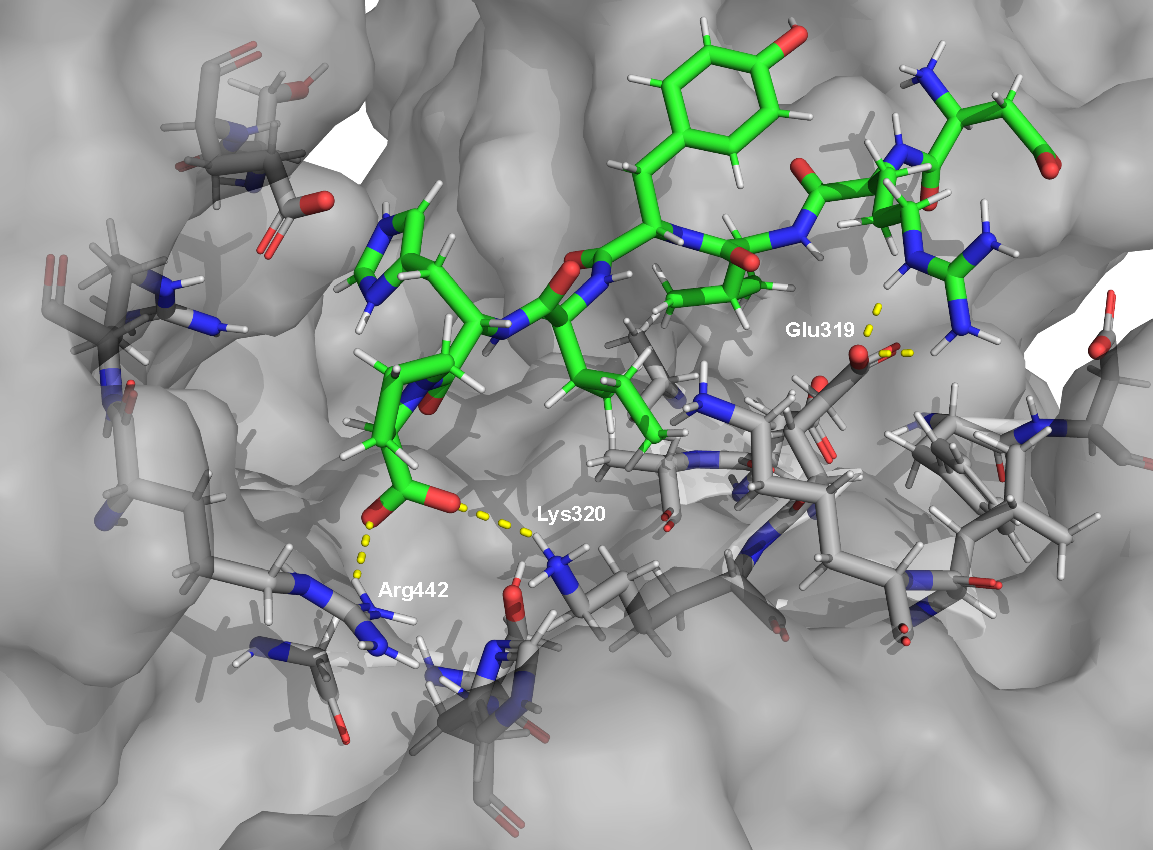
\includegraphics[width=0.9\textwidth]{last_frame_render_annotated.pdf}
  \end{center}
  \caption{\textbf{Visualisation of EOS100380 inside the binding pocket at the end of 100 ns simulation.} The polar interactions are marked with yellow dotted lines. The amino acids involved in these interactions are labelled.}\label{MD.Annotated}
\end{figure}
The figure clearly demonstrated, that the top scoring compound of our Glide screening stayed inside of the binding pocket until the end of the simulation. This was also confirmed by manual inspection of the frames generated in the simulation, which were combined to a video file using \textit{VMD}. Furthermore, the polar interactions between the ligand and residues in its proximity are shown. It seems, that EOS100380 is bound to the protein by interactions with Glu319, Lys320 and Arg442 of the NSP13 helicase. These interactions could also be validated using \textit{LigPlot+} \cite{LigPlot}.\\
To investigate the dynamics of these interactions between ligand and protein, the \ac{RMSD} and \ac{RMSF} were calculated, which can be observed in Figure~\ref{rms}. 
\begin{figure}[h]
  \begin{center}
    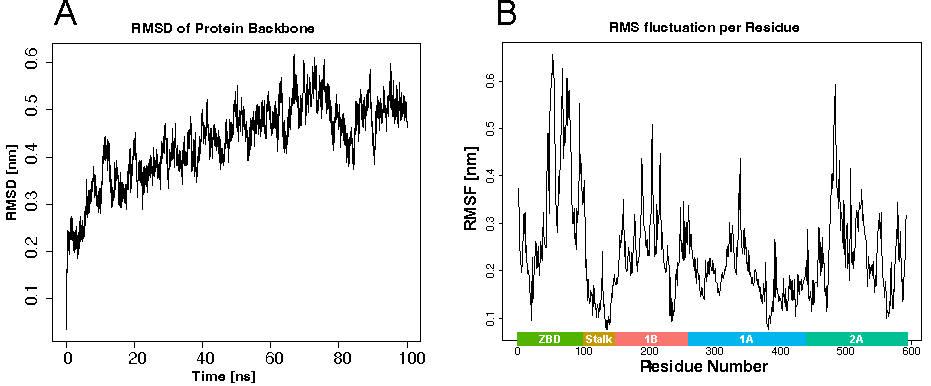
\includegraphics[width=1.0\textwidth]{RMS_Protein.pdf}
  \end{center}
  \caption{\textbf{RMSD and RMSF of the protein backbone during the simulation.} The RMSD was plotted over time for the whole 100 ns simulation. The RMSF is shown per residue. The colour bar annotates the protein domain the respective residue belongs to, according to \textcite{Domains}. ZBD = Zinc Binding Domain}
  \label{rms}
\end{figure}
The \ac{RMSD} observed over the course of the simulation (Figure~\ref{rms}A) rises at first, but reaches a plateau after roughly 60 ns. The RMSD seems to settle at roughly 0.5 nm, which is slightly larger than expected. Investigation into the RMSF per residue (Figure~\ref{rms}B) suggests, that some residues move significantly more than others. The highly mobile residues seem to be located in the zinc binding domain and domains 1B and 2A. The latter two play a role in the binding of the ligand. Thus movement in these parts of the protein was to be expected. All in all, the protein seems to undergo conformational changes, however it does not show major signs of instability. Further proof of this behaviour can be seen when investigating the radius of gyration (Supplementary Figure \ref{gyr}). The estimation of the binding energy by MMPBSA returned a $\Delta G_{solv} = -9.98 \frac{\textrm{kcal}}{\textrm{mol}}$. The RMSD and RMSF of the simulation using ANP as the ligand can be seen in Supplementary Figure \ref{anp}. The system shows a generally lower RMSD and an earlier plateau compared to the first simulation. For the RMSF a similar trend can be obeserved, especially looking at the ZBD. 
%renew after cs2

\FloatBarrier

\section{Discussion and Outlook}

The investigation into the \acf{MD} simulation further validated the viability of our pipeline. The RMSD of the backbone protein atoms (see Figure~\ref{rms}A) was slightly higher than anticipated, as it seemed to generally be smaller in the tutorials provided by \citeauthor{Lemkul2018}. However, the system stabilised over the duration of the simulation. Looking at the RMSF per residue (see Figure~\ref{rms}B) it is apparent, that certain domains of the protein lead to this increase in the RMSD. Especially the zinc binding domain shows a lot of movement. When discussing the general movement of domains in such simulations one should keep in mind, that the NSP13 A-chain is part of a much bigger replication complex \cite{NSP13_basics} in an \textit{in-vitro} setting. The conformational changes seen in this analysis would be severely hindered by other components in the complex. The domains 1B and 2A were suspected to be involved in a lot of conformational changes, as they make up a large part of the interaction surface between the protein and the ligand. The RMSD is calculated versus the output of Glide as a reference structure. It is completely possible that the system created by Glide is not completely relaxed. Thus conformational changes are to be expected when protein and ligand can suddenly move freely. Comparing the simulation with our top scoring ligand to the one with ANP shows less movement in the ANP run. This was to be expected, as ANP is very close to the original ligand of the helicase (ATP). Furthermore, the crystal structure used as input for the second run already had the ANP bound to begin with. This leads to a more relaxed starting point in general. Comparing RMSD and RMSF however, shows similarities, especially regarding the mobility of the ZBD. This further strengthens our confidence in our pipeline.  All in all, the analysis offers confidence, that EOS100380 binds to the NSP13 helicase and stays bound through an extended period of time.



\section{Limitations of the project}
Regarding the \acf{MD} simulation, the project was held back by the tight time schedule of the Meet-EU seminar. Running simulations for other top scoring ligands would have helped immensely in validating out pipeline further and compare the results of the top scorer. Running multiple runs of the same simulation would have also further deepened our confidence in the results, as MD simulations in and of them selves are a very stochastic process and should always be estimated using replicas. Following the work of \textcite{REDS}, implementing replica exchange with dynamical scaling would have elevated the validation step of this project. Access to more GPUs would have also made multiple simulations at once possible. 
Furthermore, the original plan to implement \textit{AutoGrow4} \cite{packageAutogrow4} in order to improve our lead drugs and generate novel compounds was hindered by technical problems, which could not be fixed with the limited time at our disposal. We believe, that the increase in diversity amongst the drug candidates would lead to a better final drug candidate. With the help of \textit{eToxPred}, as shown in this report, the new compounds could have been evaluated for their toxicity and a well binding, not too cytotoxic lead could have been presented. 

\pagebreak
\section{Supplementary Material}

\setcounter{figure}{0}
\renewcommand{\thefigure}{S\arabic{figure}}
\begin{figure}[h]
  \begin{center}
    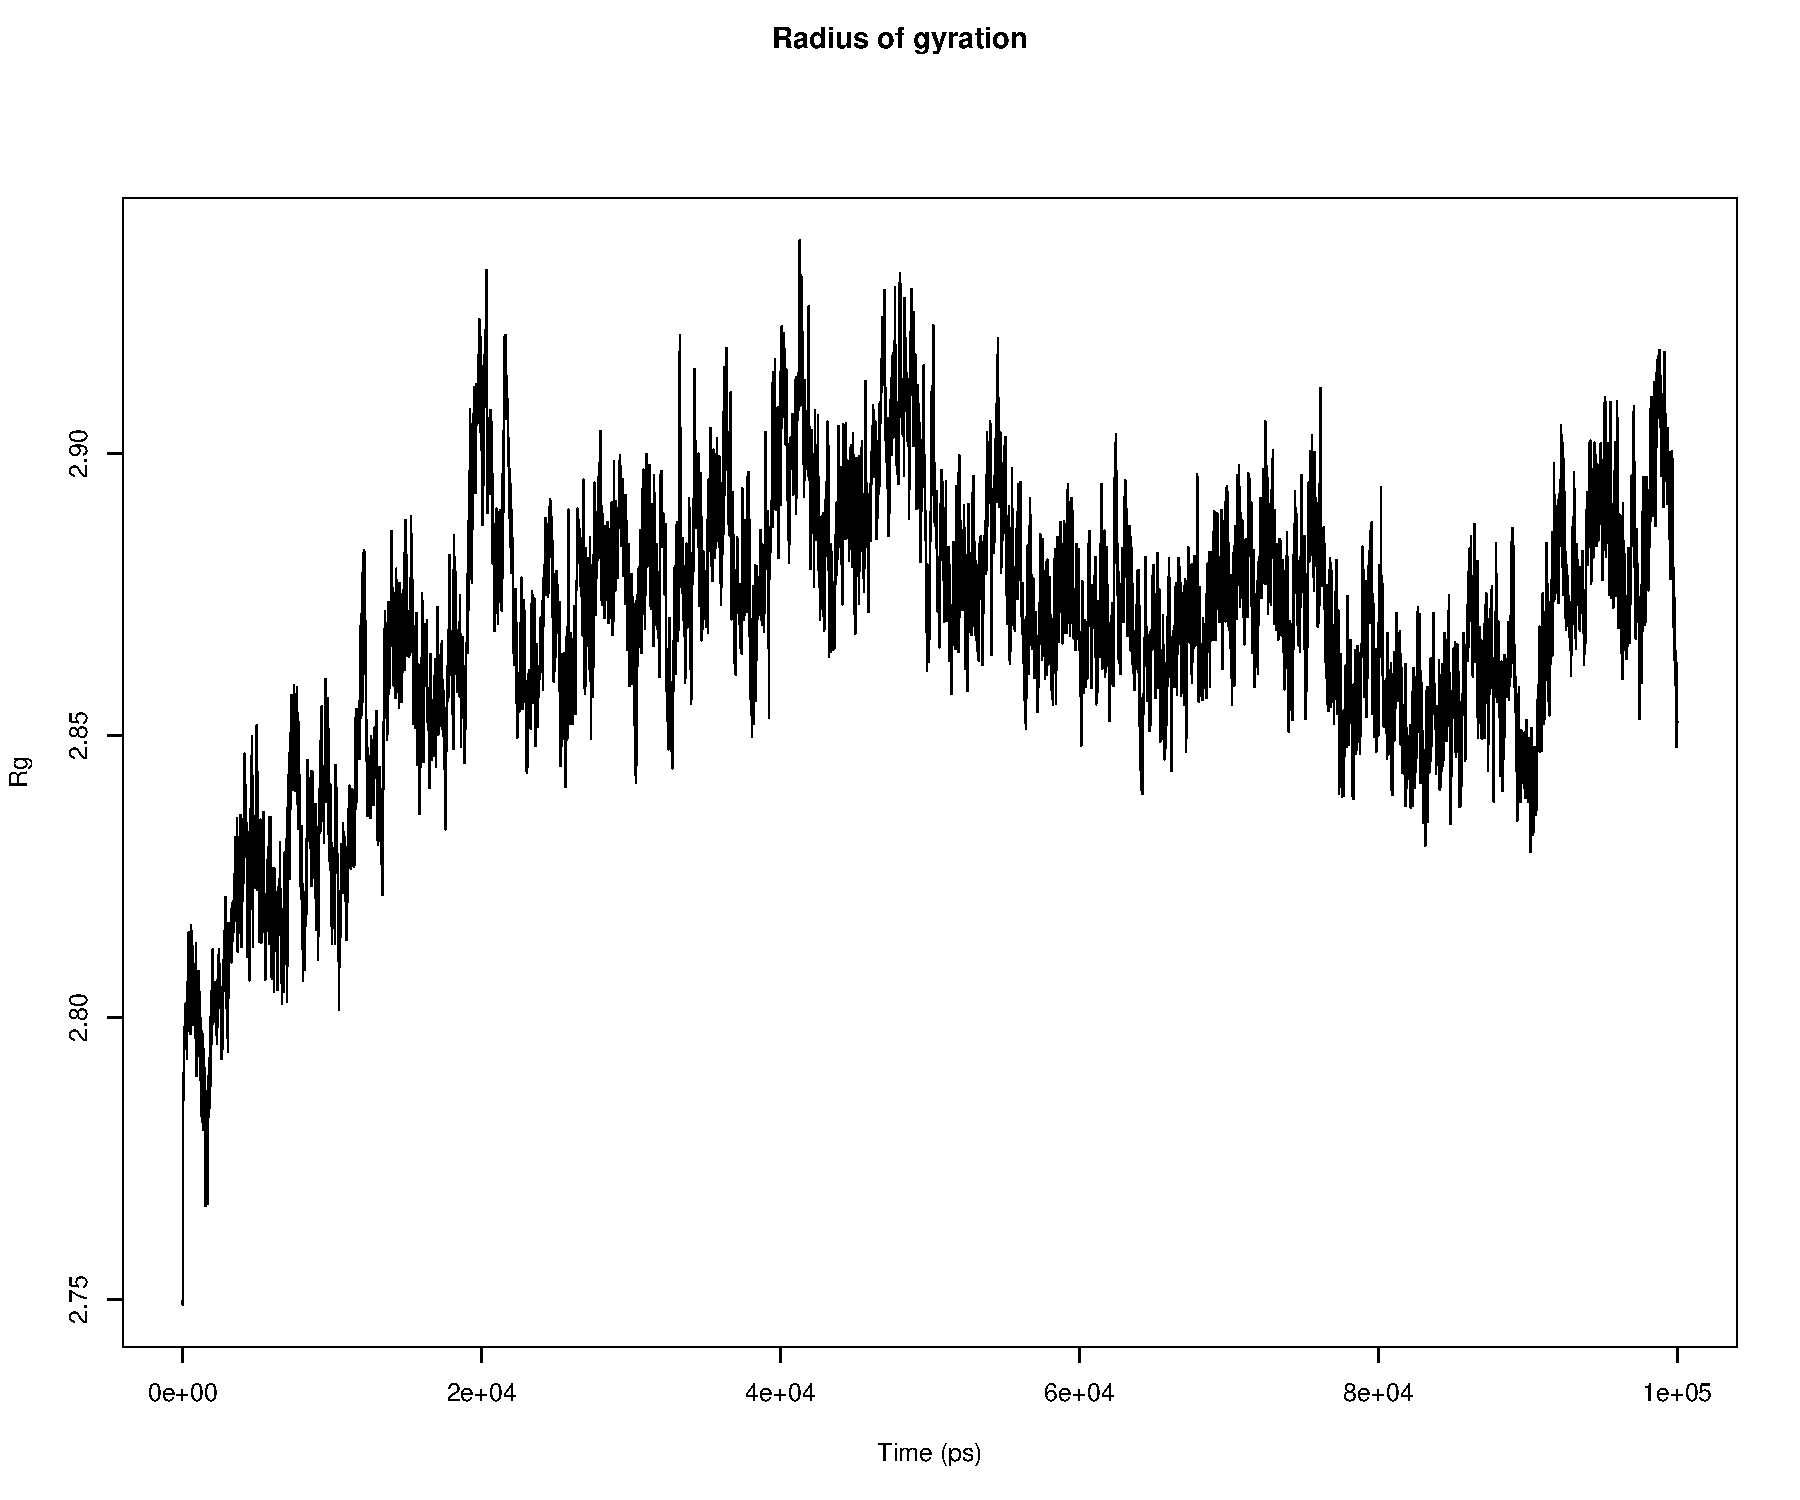
\includegraphics[width=0.7\textwidth]{gyration_protein.pdf}
  \end{center}
  \caption{Radius of Gyration of the NSP13 protein throught the production run featuring EOS100380.}\label{gyr}
\end{figure}

\begin{figure}[h]
  \begin{center}
    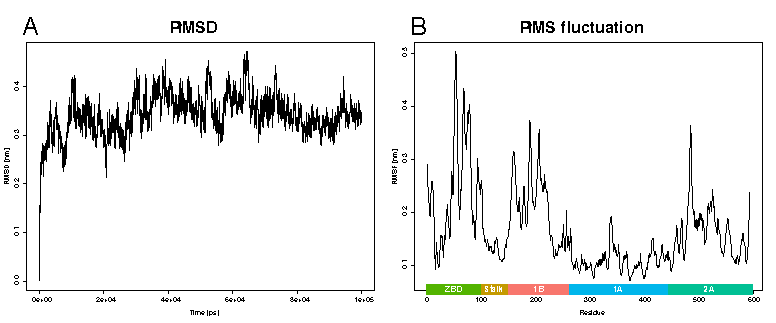
\includegraphics[width=0.95\textwidth]{rms_ANP.pdf}
  \end{center}
  \caption{RMSD and RMSF of Protein backbone for the simulation with ANP}\label{anp}
\end{figure}



\pagebreak
\FloatBarrier
\renewcommand{\bibname}{References}  % damit Literatuverzeicnis mit "References" betitelt
\printbibliography


\end{document}
